\tikzset{every picture/.style={line width=0.75pt}} %set default line width to 0.75pt        

\begin{tikzpicture}[x=0.75pt,y=0.75pt,yscale=-1,xscale=1]
%uncomment if require: \path (0,319); %set diagram left start at 0, and has height of 319

%Image [id:dp6954457554746387] 
\draw (280.94,160.96) node  {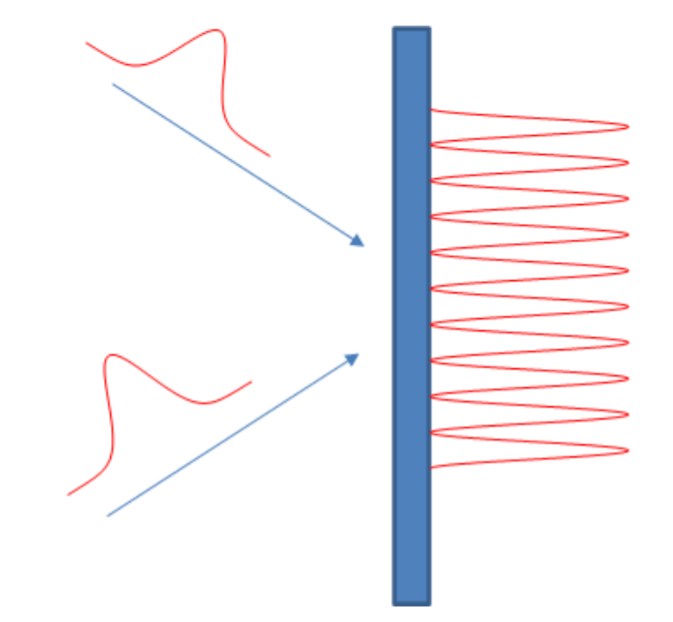
\includegraphics[width=162.44pt,height=162.44pt]{problem-1-detector.PNG}};
%Straight Lines [id:da9771961350544831] 
\draw    (138,41.86) -- (443.02,41.86) ;
\draw [shift={(445.02,41.86)}, rotate = 180] [fill={rgb, 255:red, 0; green, 0; blue, 0 }  ][line width=0.08]  [draw opacity=0] (12,-3) -- (0,0) -- (12,3) -- cycle    ;
%Straight Lines [id:da46670676444957326] 
\draw    (138,281) -- (138,41.86) ;
\draw [shift={(138,283)}, rotate = 270] [fill={rgb, 255:red, 0; green, 0; blue, 0 }  ][line width=0.08]  [draw opacity=0] (12,-3) -- (0,0) -- (12,3) -- cycle    ;

% Text Node
\draw (447.02,41.86) node [anchor=west] [inner sep=0.75pt]    {$z$};
% Text Node
\draw (138,286.4) node [anchor=north] [inner sep=0.75pt]    {$x$};


\end{tikzpicture}